\documentclass{article}

\usepackage{fullpage}  % Makes the text margins smaller
\usepackage{graphicx} % To include figures
\usepackage{fancyvrb} % Includes the \VerbatimInput command to read in code files

\author{Cody Lieu, Yixin Lin}
\title{COMPSCI 527 Homework 4}

\begin{document}
\maketitle

\section*{Problem 1(a)}

\VerbatimInput[fontsize=\small,fontshape=n,xleftmargin=15mm]{nn.m}

\section*{Problem 1(b)}

\VerbatimInput[fontsize=\small,fontshape=n,xleftmargin=15mm]{approximator.m}

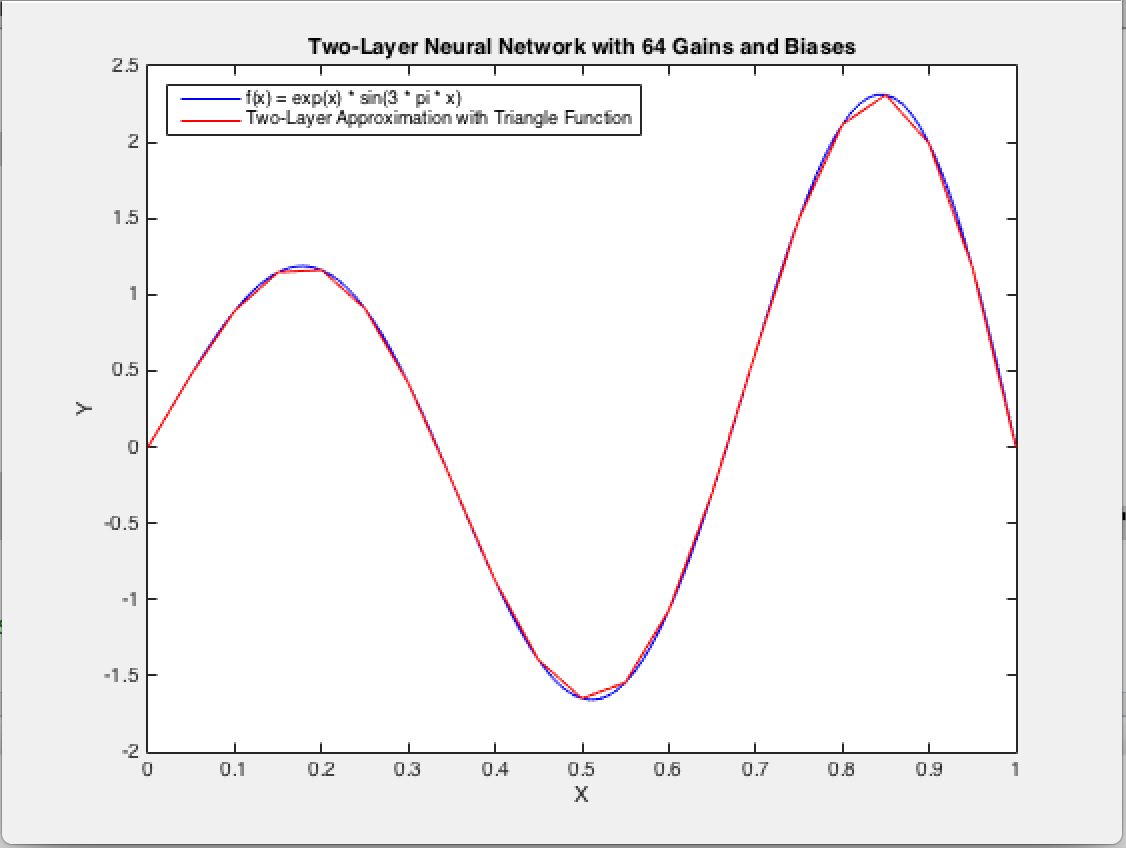
\includegraphics[width=0.8\textwidth]{1b.png}

\section*{Problem 1(c)}

$n_w = 3K + 1$

\section*{Problem 2(a)}

$p = m - n + 1$

\section*{Problem 2(b)}

\[
C_v(\textbf{k}) = \left[\begin{array}{*{7}c}
 k_3 & k_2 & k_1 &  &  &  & \\
 & k_3 & k_2 & k_1 & & &\\
 &  & k_3 & k_2 & k_1 & & \\
 &  &  & k_3 & k_2 & k_1 &\\
 & & & & k_3 & k_2 & k_1
\end{array}\right]
\]

\[
C_f(\rho(\textbf{k})) = \left[\begin{array}{*{5}c}
 k_3 &  &  & & \\
 k_2 & k_3 &  & & \\
 k_1 & k_2 & k_3 & & \\
 & k_1 & k_2 & k_3 &\\
  & & k_1 & k_2 & k_3 \\
 &   & & k_1 & k_2 \\
  & &  & & k_1\\
\end{array}\right]
\]\\\\

$a(\textbf{x}) = \textbf{x} \ast_v \textbf{k} + b$\\

$a(\textbf{x}) = C_v(\textbf{k})\textbf{x} + b$\\

Differentiate both sides:\\

$A_\textbf{x} = C_v(\textbf{k})$\\

$A_\textbf{x}^T = C_v(\textbf{k})^T$\\

$A_\textbf{x}^T = C_f(\rho(\textbf{k}))$\\

$e_\textbf{x} = A_\textbf{x}^Te_\textbf{a}$\\

$e_\textbf{x} = C_f(\rho(\textbf{k}))e_\textbf{a}$\\

$e_\textbf{x} = e_\textbf{a} \ast_f \rho(\textbf{k})$

\section*{Problem 2(c)}

$\textbf{a}' = \sigma_r(\textbf{a}(\textbf{x}), 2) = [a_1, a_3, a_5]^T$\\

$e_\textbf{a}' = \sigma_r(\textbf{a}(\textbf{x}), 2) = [e_{a1}, e_{a3}, e_{a5}]^T$\\

$e_\textbf{x}' = \delta(e_\textbf{a}', p) \ast_f \rho(\textbf{k})$\\

$e_\textbf{x}' = C_f(\rho(\textbf{k}))\delta(e_\textbf{a}', p)$\\

$e_\textbf{x}' = C_v(\textbf{k})^T\delta(e_\textbf{a}', p)$\\

$e_\textbf{x}' = A_\textbf{x}^T\delta(e_\textbf{a}', p)$\\

The original equivalence of $e_\textbf{x} = A_\textbf{x}^Te_\textbf{a}$ becomes $e_\textbf{x}' = \sigma_r(A_\textbf{x}, 2)^Te_\textbf{a}'$, which makes sense since every 2nd row of $A_\textbf{x}$ is removed in the matrix multiplication with the transpose of $A_\textbf{x}$ since every 2nd row of $e_\textbf{a}$ was removed with the row sampling operator. These two expressions result in the equivalence below:\\

$A_\textbf{x}^T\delta(e_\textbf{a}', p) = \sigma(A_\textbf{x}, 2)^Te_\textbf{a}'$\\

This equivalence makes intuitive sense. On the left-hand side of the expression, we have the transpose of the Jacobian multiplied by $e_\textbf{a}$ after being row-sampled with a stride of 2 and then diluted to p. This means that the left-hand side of the expression is equivalent to $A_\textbf{x}^Te_\textbf{a}$ from part b except every 2nd column of $A_\textbf{x}^T$ (2nd row of $A_\textbf{x}$) contributes nothing to the result. On the right-hand side of the expression, we row-sample $A_\textbf{x}$ by 2 and then multiply the transpose of that with $e_\textbf{a}'$, which implicitly ignores every second row of the original $e_\textbf{a}$ and uses every second column of $A_\textbf{x}^T$ just like the left-hand side. An alternative proof is shown below:\\

$a(\textbf{x}) = \textbf{x} \ast_v \textbf{k} + b$\\

$\sigma_r(a(\textbf{x}), 2) = \sigma_r(\textbf{x} \ast_v \textbf{k} + b, 2)$\\

This equivalence is apparent from drawing out the row-sampled versions of the matrices from part b.\\

$\sigma_r(a(\textbf{x}), 2) = \sigma_r(C_v(\textbf{k})\textbf{x} + b, 2)$\\

Differentiate both sides, which is still possible because they're matrices:\\

$\sigma_r(A_\textbf{x}, 2) = \sigma_r(C_v(\textbf{k}), 2)$\\

Using the equality from part b:\\

$\sigma_r(A_\textbf{x}, 2) = \sigma_r(A_\textbf{x}, 2)$\\

\section*{Problem 3(a)}

\VerbatimInput[fontsize=\small,fontshape=n,xleftmargin=15mm]{cnn.m}

$y = [534.6887, 130.5719, 347.6032, 0.1243, 759.6464]$

$e = 1.2245$

\section*{Problem 3(b)}

\VerbatimInput[fontsize=\small,fontshape=n,xleftmargin=15mm]{backprop.m}

\section*{Problem 3(c)}

\VerbatimInput[fontsize=\small,fontshape=n,xleftmargin=15mm]{numeric.m}

\section*{Problem 3(d)}

\VerbatimInput[fontsize=\small,fontshape=n,xleftmargin=15mm]{ee2.m}


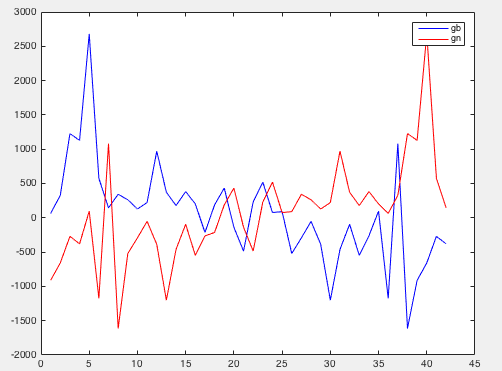
\includegraphics[width=0.8\textwidth]{graph1.png}
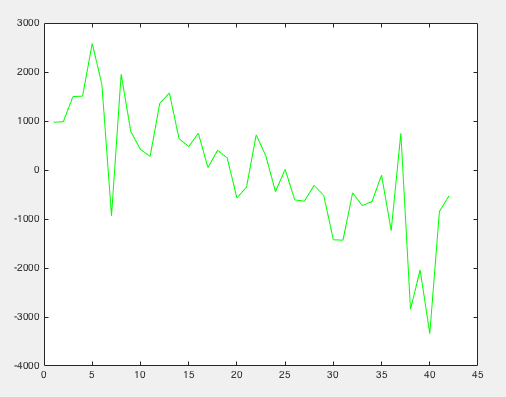
\includegraphics[width=0.8\textwidth]{graph2.png}

ndg = 1.6721

\end{document}
